% ------------------------------------ ANALISI ----------------------------------

\chapter{Analisi}

\textsf{\small \textbf{Bullet Ballet} è un videogioco platform a scorrimento orizzontale, del genere \emph{Shoot 'em up} in 2D.}\\
\textsf{\small L'obiettivo del gioco è quello di realizzare più punti possibili per superare i propri record, in base alla distanza percorsa dal giocatore.}\\

\textsf{\small Ma non sarà tutto in discesa, il giocatore dovrà affrontare nemici con i più variegati equipaggiamenti, ostacoli di ogni sorta, varchi nella mappa e molto altro ancora..}\\
\textsf{\small Il giocatore potrà scegliere fra ben 8 mappe uniche e relative piattaforme in tema.}\\

\textsf{\small Inoltre, il giocatore potrà avvalersi a sua volta di effetti (bonus) sia positivi che negativi per poter sconfiggere le avversità che si presenteranno sul suo cammino.}\\

\textsf{\small Potrà, poi salvare tutti i suoi punteggi di gioco.}\\

\begin{comment}
In questo capitolo andrà fatta l'analisi dei requisiti e quella del problema, ossia verranno elencate le cose che l'applicazione dovrà fare (requisiti) e verrà descritto il dominio applicativo (analisi del problema).
%
In fase di analisi, è molto importante tenere a mente che non vi deve essere alcun riferimento al design né tantomeno alle tecnologie implementative, ovvero, non si deve indicare come il software sarà internamente realizzato.
%
La fase di analisi, infatti, \textit{precede} qualunque azione di design o di implementazione.
\end{comment}

\section{Requisiti}

\textsf{\small L'applicazione mostra, all'avvio, un menù di gioco con le seguenti voci: \emph{New Game}, \emph{Load Game}, \emph{Settings},\emph{Quit}.}\\

\begin{comment}
Nell'analisi dei \emph{requisiti} dell'applicazione si dovrà spiegare cosa l'applicazione dovrà fare.
%
Non ci si deve concentrare sui particolari problemi, ma esclusivamente su cosa si desidera che l'applicazione faccia.
%
È consigliato descrivere separatamente i requisiti funzionali (quelli che descrivono l'effettivo
comportamento dell'applicazione) da quelli non funzionali (requisiti che non riguardano direttamente
aspetti comportamentali, come sicurezza, performance, eccetera).
\end{comment}

\begin{comment}
\subsection*{Elementi positivi}
\begin{itemize}
	\item Si fornisce una descrizione in linguaggio naturale di ciò che il software dovrà fare.
	\item Gli obiettivi sono spiegati con chiarezza, per punti.
	\item Se il software è stato commissionato o è destinato ad un utente o compagnia specifici, il committente viene nominato.
	\item Se vi sono termini il cui significato non è immediatamente intuibile, essi vengono spiegati.
	\item Vengono descritti separatamente requisiti funzionali e non funzionali.
	\item Considerato a un paio di pagine un limite ragionevole alla lunghezza della parte sui requisiti, in quello spazio si deve cercare di chiarire \textit{tutti} gli aspetti dell'applicazione, non lasciando decisioni che impattano la parte ``esterna'' alla discussione del design (che dovrebbe solo occuparsi della parte ``interna'').
\end{itemize}

\subsection*{Elementi negativi}
\begin{itemize}
	\item Si forniscono indicazioni circa le soluzioni che si vogliono adottare
	\item Si forniscono dettagli di tipo tecnico o implementativo (parlando di classi, linguaggi di programmazione, librerie, eccetera)
\end{itemize}

\subsection*{Esempio}
Il software, commissionato dal gestore del centro di ricerca ``Aperture Laboratories Inc.''\footnote{\url{http://aperturescience.com/}}, mira alla costruzione di una intelligenza artificiale di nome GLaDOS (Genetic Lifeform and Disk Operating System).
%
Per intelligenza artificiale si intende un software in grado di assumere decisioni complesse in maniera semi autonoma sugli argomenti di sua competenza, a partire dai vincoli e dagli obiettivi datigli dall'utente.
\end{comment}

\subsubsection{Requisiti funzionali}

\begin{itemize}
	\item \textsf{\small \emph{Mappa scorrevole}: Il giocatore potrà muoversi in una mappa a scorrimento orizzontale con uno sfondo statico.}
	\item \textsf{\small \emph{Menù di gioco}: Non appena lanciata l'applicazione, l'utente vedrà un menù di gioco con diverse opzioni tra cui potrà scegliere.}
	\item \textsf{\small \emph{Menù di pausa}: Il giocatore potrà mettere il gioco in pausa attraverso un dato pulsante della tastiera, scelto nelle impostazioni.}
	\item \textsf{\small \emph{Personaggio}: Il giocatore potrà scegliere un personaggio e muoverlo in partita.}
	\item \textsf{\small \emph{Nemici}: Verranno generati diversi nemici che il giocatore dovrà affrontare.}
	\item \textsf{\small \emph{Ostacoli e oggetti raccoglibili}: Verranno creati nella mappa degli ostacoli che bloccheranno la strada e degli oggetti che il giocatore potrà raccogliere per ricevere un (power up) bonus od un malus.}
	\item \textsf{\small \emph{Salvataggio del punteggio e classifica}: Terminata la partita, il punteggio di gioco potrà essere salvato e verrà generata una classifica finale.}
	\item \textsf{\small \emph{Suoni ed effetti sonori}: La durata della partita verrà accompagnata da una colonna sonora e agli effetti sonori prodotti dall'environment di gioco.}
	\item \textsf{\small \emph{Fisica di gioco}: Tutti le entità di gioco saranno dotati di una fisica ed una gravità propria.}
	%\item \textsf{\small }
	%\item \textsf{\small }
	%\item \textsf{\small }
	%\item \textsf{\small }
\end{itemize}

\begin{comment}
\begin{itemize}
\item La suddetta intelligenza artificiale dovrà occuparsi di coordinare le attività all'interno
delle camere di test di Aperture, guidando l'utente attraverso un certo numero di sfide di
difficoltà crescente. Una camera di test è un ambiente realizzato da Aperture Laboratories Inc. al
fine di mettere alla prova le proprie tecnologie di manipolazione dell'ambiente. All'interno della
camera di test, un soggetto qualificato è incaricato di sfruttare gli strumenti messi a
disposizione da Aperture per risolvere alcuni rompicapi. I rompicapi sono di tipo fisico (ad
esempio, manipolazione di oggetti, pressione di pulsanti, azionamento di leve), e si ritengono
conclusi una volta che il soggetto riesce a trovare l'uscita dalla camera di test.
\item Il piano preciso ed il numero delle sfide sarà variabile, e GLaDOS dovrà essere in grado di adattarsi dinamicamente e di fornire indicazioni di guida.
\item La personalità di GLaDOS dovrà essere modificabile.
\item GLaDOS dovrà essere in grado di comunicare col reparto cucina di Aperture, per ordinare torte da donare agli utenti che completassero l'ultima camera di test con successo.
\end{itemize}
\end{comment}

%\subsubsection{Requisiti non funzionali}
\subsection{Requisiti opzionali}

\textsf{\small Questi requisiti non concorrono a far parte delle funzionalità minime del gioco e per questioni di tempistica e/o di budget non verranno necessariamente implementate.}\\

\begin{itemize}
	\item \textsf{\small \emph{Oggetti dinamici}: ovvero oggetti che si muovono e che hanno una animazione.}
	\item \textsf{\small \emph{Market}: per poter comprare/vendere skin (mimetiche) di gioco con valuta reale o in gioco. (o fittizia del gioco)}
	\item \textsf{\small \emph{Modalità storia}: una modalità con una storia di gioco e diversi livelli che il giocatore dovrà sbloccare per poter continuare ad avanzare nel gioco.}
	\item \textsf{\small \emph{Statistiche di gioco}: Varie statistiche di gioco, mostrate in diversi diagrammi.}
	\item \textsf{\small \emph{Difficoltà di gioco}: Possibilità di scegliere diverse difficoltà che potrebbero aggiungere numero di nemici/ostacoli/oggetti di varia natura e/o incrementare la loro vita.}
	%\item \textsf{\small }
\end{itemize}

\begin{comment}
\begin{itemize}
\item GLaDOS dovrà essere estremamente efficiente nell'uso delle risorse. Le specifiche tecniche parlano della possibilità di funzionare su dispositivi alimentati da una batteria a patata.
\end{itemize}
\end{comment}

\section{Analisi e modello del dominio}

\textsf{\small L'applicazione fornisce un giocatore che tramite input dell'utente può essere spostato a destra, a sinistra e farlo saltare. Il quale, potrà interagire con le varie entità, sia statiche che dinamiche del gioco, quali \emph{nemici}, \emph{armi}, \emph{monete}, \emph{items}, \emph{ostacoli}.
Ognuna di queste entità interagirà in maniere differenti col player: }\\

\begin{itemize}
	\item \textsf{\small \emph{Enemy}, ostacolerà il player a colpi di mitra.} %TODO: da modificare.
	\item \textsf{\small \emph{Item}, una volta raccolta dal player, gli fornirà o un \textbf{bonus}, come una vita extra oppure un \textbf{malus} come un effetto di volevo per tot tempo.}
	\item \textsf{\small \emph{monete}, faranno aumentare il punteggio e il numero di monete del gioco da usare nel mercato per poter comprare nuove skins, in game-items, ecc..}
	\item \textsf{\small \emph{Armi}, dopo essere state raccolte verranno equipaggiate al giocatore.}
	\item \textsf{\small \emph{Ostacoli}, se il player ci colliderà, subirà del danno.}
\end{itemize}

\textsf{\small Il gioco si conclude quando e se il player riesce a raggiungere la fine della mappa senza morire.}
\textsf{\small Se il player viene ucciso prima di raggiungere la fine, allora viene eliminato e la partita è persa.}\\

\textsf{\small Ogni round è a sè stante, finita la partita, al player verrà assegnato un punteggio e potrà scegliere se rigiocare od uscire.}\\

%TODO: aggiungere UML.

%\begin{landscape}
	\begin{figure}[h]
		\centering{}
		%\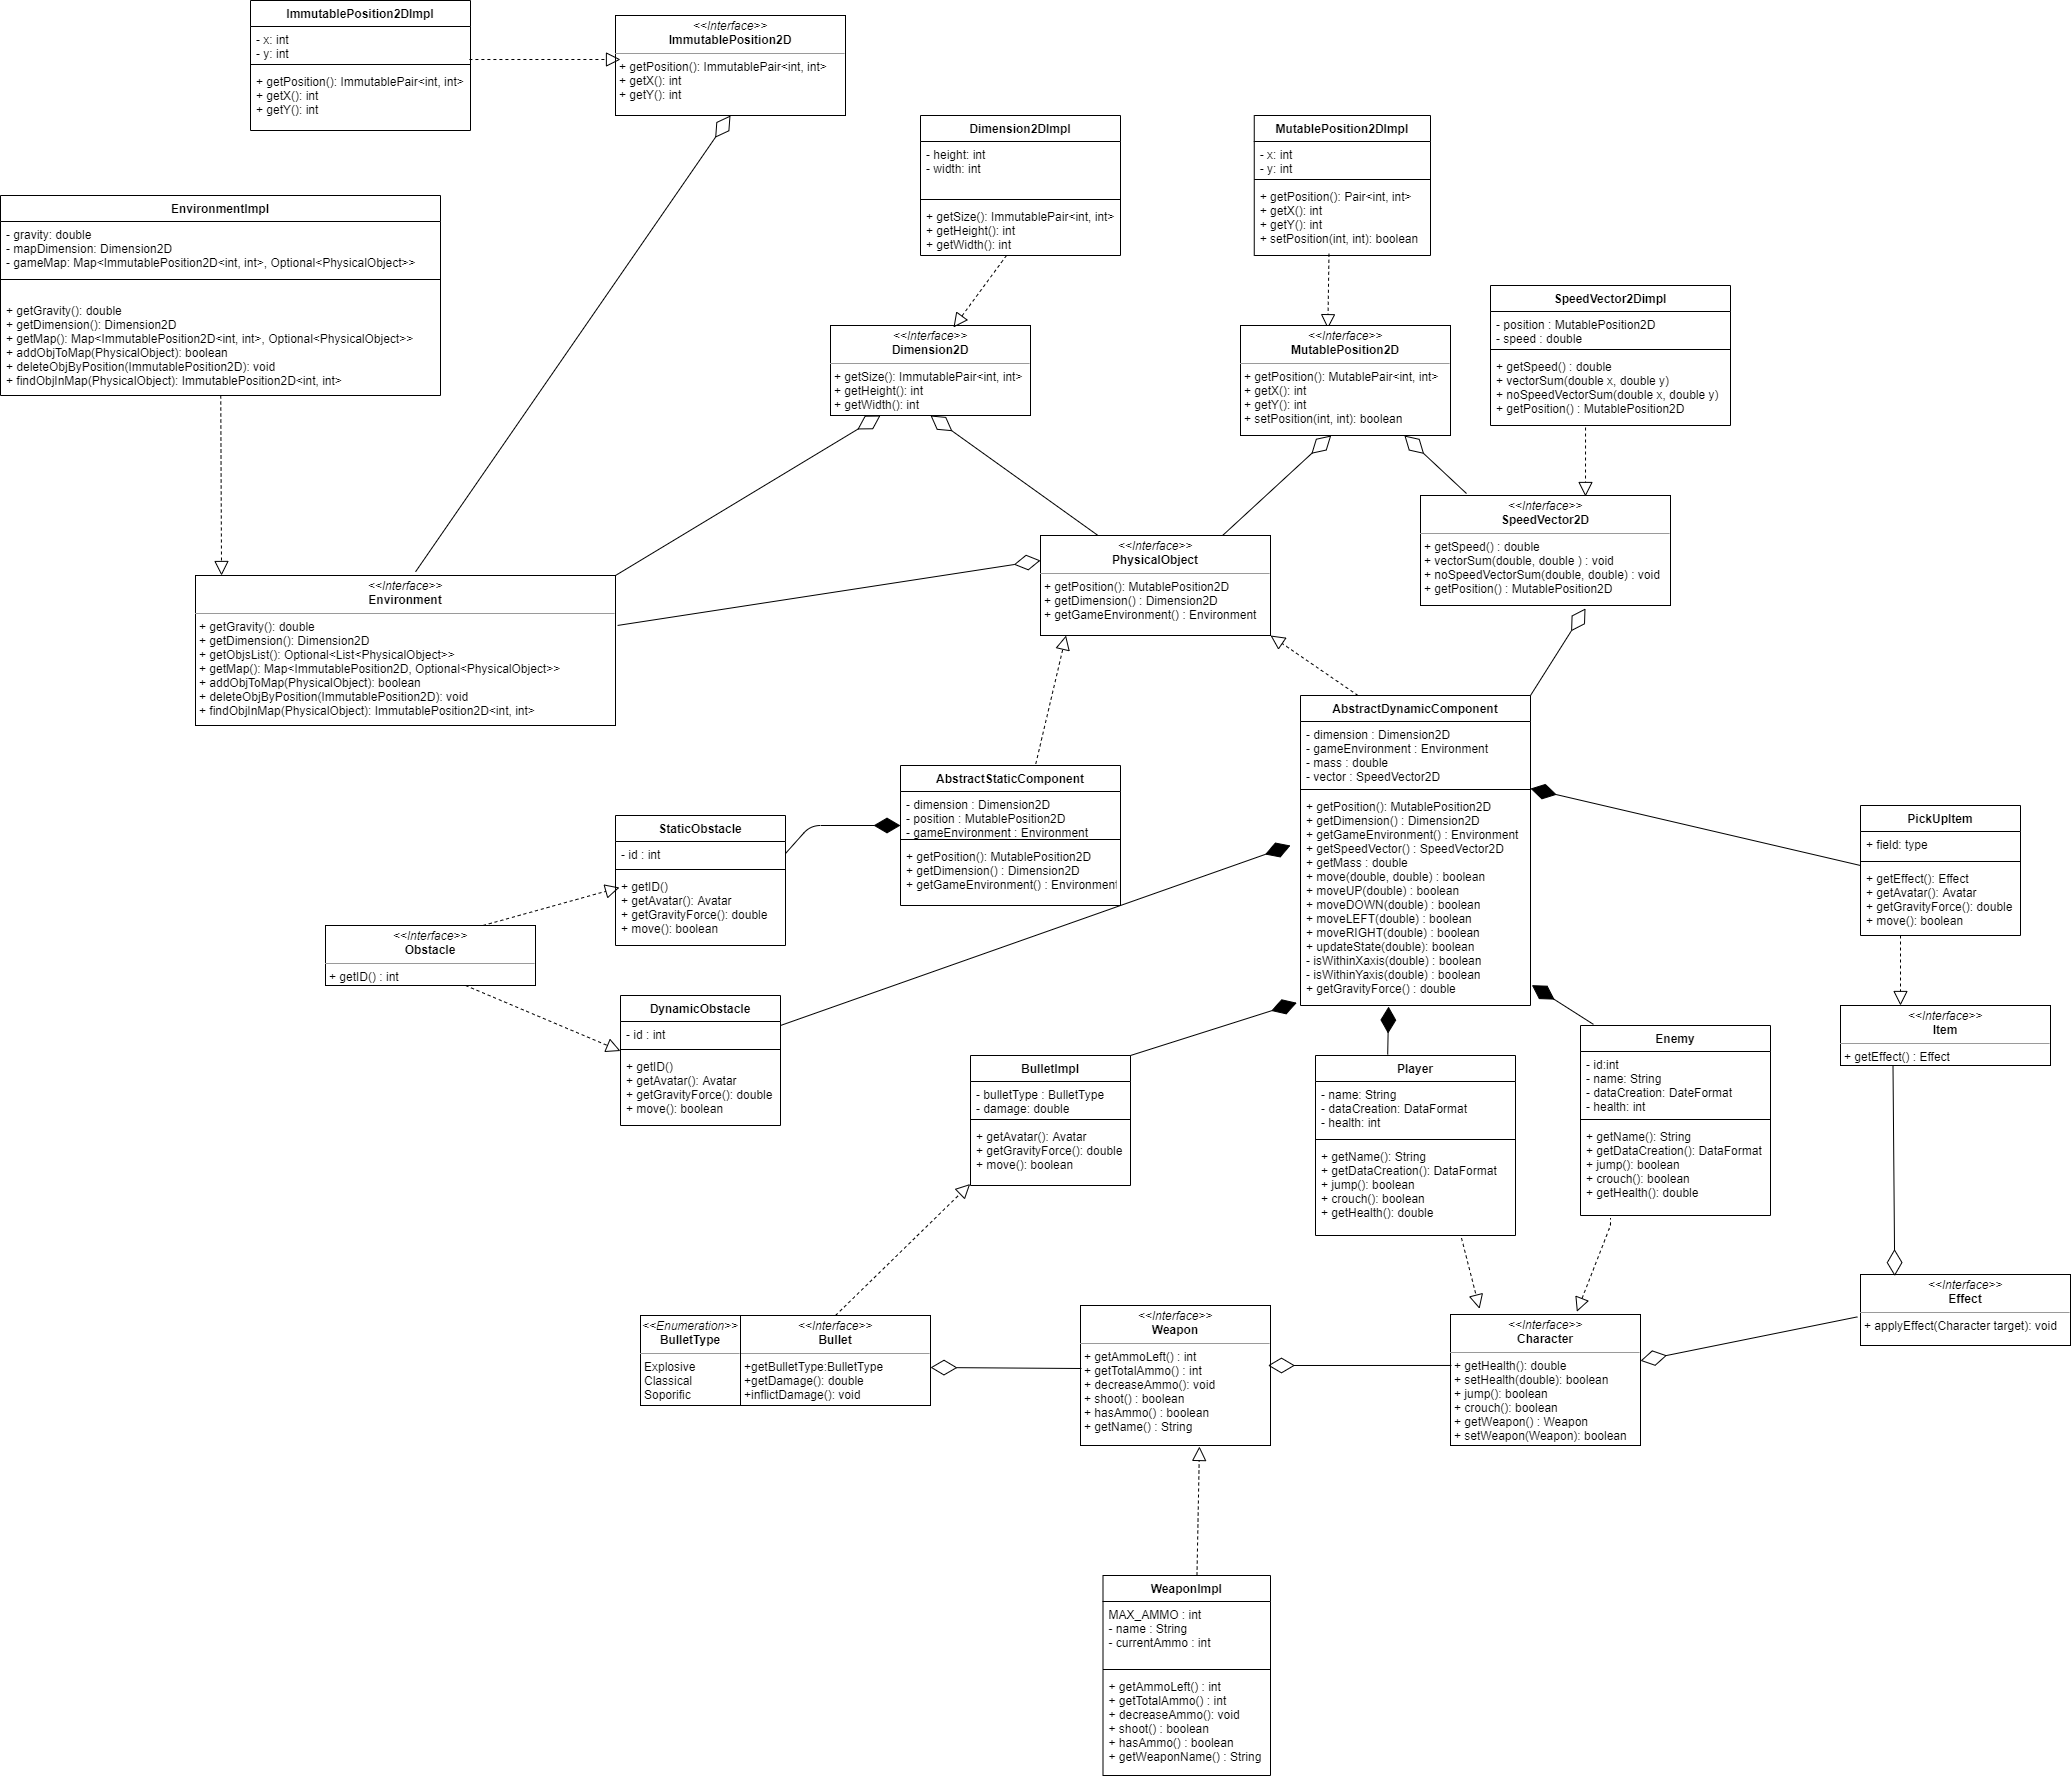
\includegraphics[width=1.2\linewidth]{./img/model.png} %TODO: cambiare UML
		\caption{Schema UML dell'analisi del problema, con rappresentate le entità principali ed i rapporti fra loro.}
		\label{img:analysis}
	\end{figure}
%\end{landscape}

\begin{comment}

In questa sezione si descrive il modello del \textit{dominio
	applicativo}, descrivendo le \textit{entità} in gioco ed i rapporti fra loro.
%
Si possono sollevare eventuali aspetti particolarmente impegnativi, descrivendo perché lo sono, senza inserire idee circa possibili soluzioni, ovvero sull'organizzazione interna del software.
%
Infatti, la fase di analisi va effettuata \textbf{prima} del progetto: né il progetto né il software esistono nel momento in cui si effettua l'analisi.
%
La discussione di aspetti propri del software (ossia, della \textit{soluzione} al problema e non del problema stesso) appartengono alla sfera della progettazione, e vanno discussi successivamente.

È obbligatorio fornire uno schema UML del dominio, che diventerà anche lo scheletro della
parte ``entity'' del modello dell'applicazione, ovvero degli elementi costitutivi del modello (in ottica MVC - Model View Controller): se l'analisi è ben fatta, dovreste ottenere una gerarchia di concetti che rappresentano le entità che compongono il problema da risolvere.
%
Un'analisi ben svolta \textbf{prima} di cimentarsi con lo sviluppo rappresenta un notevole aiuto per
le fasi successive: è sufficiente descrivere a parole il dominio, quindi estrarre i sostantivi
utilizzati, capire il loro ruolo all'interno del problema, le relazioni che intercorrono fra loro, e
reificarli in interfacce.

\subsection*{Elementi positivi}
\begin{itemize}
	\item Viene descritto accuratamente il modello del dominio.
	\item Alcuni problemi, se non risolubili in assoluto o nel monte ore, vengono dichiarati come problemi che non saranno risolti o sarano risolti in futuro.
	\item Si modella il dominio in forma di UML, descrivendolo appropriatamente.
\end{itemize}

\subsection*{Elementi negativi}
\begin{itemize}
	\item Manca una descrizione a parole del modello del dominio.
	\item Manca una descrizione UML delle entità del dominio e delle relazioni che intercorrono fra loro.
	\item Vengono elencate soluzioni ai problemi, invece della descrizione degli stessi.
	\item Vengono presentati elementi di design, o peggio aspetti implementativi.
	\item Viene mostrato uno schema UML che include elementi implementativi o non utili alla descrizione del dominio, ma volti alla soluzione (non devono vedersi, ad esempio, campi o metodi privati, o cose che non siano equivalenti ad interfacce).
\end{itemize}

\subsection*{Esempio}
GLaDOS dovrà essere in grado di accedere ad un'insieme di camere di test.
%
Tale insieme di camere prende il nome di percorso.
%
Ciascuna camera è composta di challenge successivi.
%
GLaDOS è responsabile di associare a ciascun challenge un insieme di consigli (suggestions) destinati all'utente (subject), dipendenti da possibili eventi.
%
GLaDOS dovrà poter comunicare coi locali cucina per approntare le torte.
%
Le torte potranno essere dolci, oppure semplici promesse di dolci che verranno disattese.

Gli elementi costitutivi il problema sono sintetizzati in \Cref{img:analysis}.

La difficoltà primaria sarà quella di riuscire a correlare lo stato corrente dell'utente e gli eventi in modo tale da generare i corretti suggerimenti.
%
Questo richiederà di mettere in campo appropriate strategie di intelligenza artificiale.

Data la complessità di elaborare consigli via AI senza intervento umano, la prima versione del software fornita prevederà una serie di consigli forniti dall'utente.

Il requisito non funzionale riguardante il consumo energetico richiederà studi specifici sulle performance di GLaDOS che non potranno essere effettuati all'interno del monte ore previsto: tale feature sarà oggetto di futuri lavori.

\begin{figure}[h]
	\centering{}
	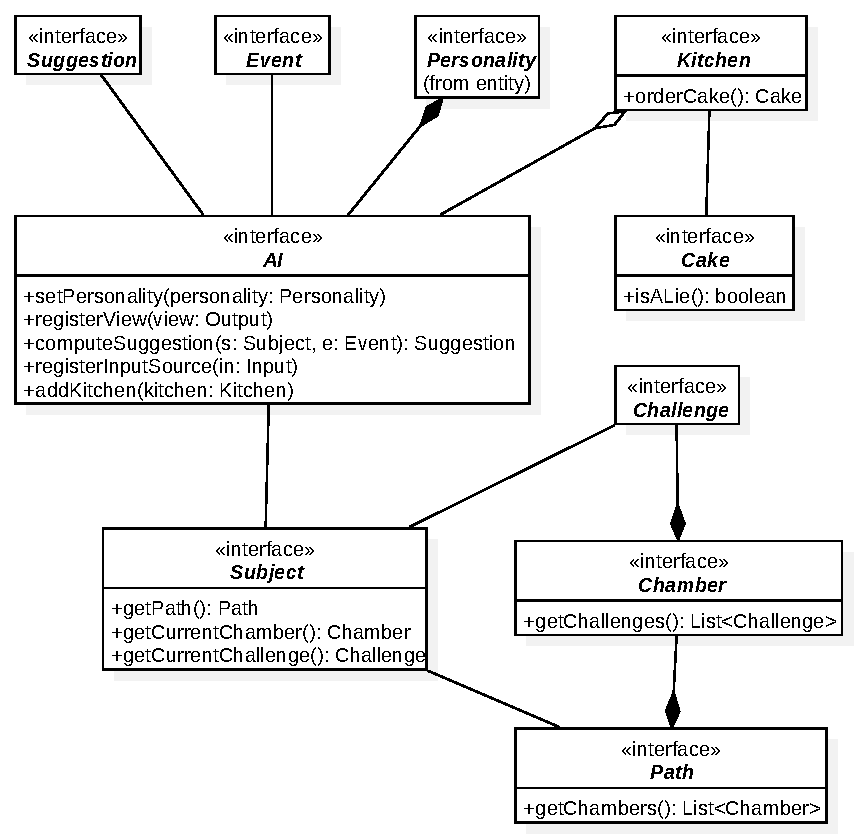
\includegraphics{img/analysis.pdf}
	\caption{Schema UML dell'analisi del problema, con rappresentate le entità principali ed i rapporti fra loro}
	\label{img:analysis}
\end{figure}

\end{comment}